\documentclass[12pt, twoside]{article}
\usepackage[francais]{babel}
\usepackage[T1]{fontenc}
\usepackage[latin1]{inputenc}
\usepackage[left=5mm, right=5mm, top=5mm, bottom=5mm]{geometry}
\usepackage{float}
\usepackage{graphicx}
\usepackage{array}
\usepackage{multirow}
\usepackage{amsmath,amssymb,mathrsfs}
\usepackage{textcomp}
\pagestyle{empty}
\usepackage{soul}
\usepackage{eurosym}


\begin{document} 



\begin{center}
{\fbox{$6^{e} \ldots $ \qquad \qquad \textbf{\Large{Devoir surveill� 4 }}
\qquad \qquad 16/01/2014}}
\end{center}



\enskip


\textit{Remarque: Tous les exercices sont � faire sur votre feuille.}

\medskip


\ul{Exercice 1}: (\textit{2,5 points})

\begin{enumerate}
  \item Recopier et compl�ter: 4,6 et \ldots sont les \ldots\ldots de la
  multiplication 4,6 $\times $ 34,5.
  \item Comment s'appelle le r�sultat d'une multiplication?
  \item Calculer la somme de 64,56 et de 19.
  \item Calculer le triple de 15.
\end{enumerate}

\bigskip

\ul{Exercice 2}: (\textit{4 points}) Poser et effectuer:

\enskip

$453,3+48,97$ \qquad \qquad \qquad $724-148,36$ \qquad \qquad \qquad $18,6
\times 9,7$ \qquad \qquad \qquad $84,2 \times 2,06$


\bigskip

\ul{Exercice 3}: (\textit{2 points})
Calculer astucieusement (d�taillez votre m�thode):

\begin{center}
$A=3,4 + 51,17+ 3,6 +13,03$ \qquad \qquad \qquad $B=0,5 \times 45,7 \times 2$
\end{center}


\bigskip


\ul{Exercice 4}: (\textit{2,5 points})

\begin{enumerate}
  \item Le train de No�mie quitte Paris � 19h41min. La dur�e de son trajet est
  2h39min. Quelle est l'heure d'arriv�e du train de No�mie?
  \item Le lendemain matin, No�mie fait une randonn�e � v�lo. Elle part �
  8h45min et elle revient � 10h26min. Combien de temps a-t-elle roul�?
\end{enumerate}



\bigskip


\ul{Exercice 5}: (\textit{2 points}) Calculer sans poser l'op�ration.

\begin{center}

a) $12,9 \times 0,1$ \qquad \qquad b) $57,8 \times 100$ \qquad \qquad c)
$528,46 \times 0,001$ \qquad \qquad d) $9,362 \times 10$

\end{center}


\bigskip


\ul{Exercice 6}: (\textit{2,5 points})

\enskip

Mathieu a achet� un livre � 4,95 \euro, un journal � 2,50 \euro et deux stylos
� 2,77 \euro l'un. Apr�s ses achats, il lui reste 3,20 \euro.

\begin{enumerate}
  \item Calculer le montant des achats de Mathieu.
  \item Combien d'argent avait Mathieu avant ses achats?
\end{enumerate}


\bigskip

\ul{Exercice 7}: (\textit{2,5 points})


\begin{tabular}{ccc}
\begin{minipage}{9cm}
Esteban, Laura, Sa�d et Kevin ont din� au restaurant. Esteban pense qu'ils
doivent payer 88,90 \euro. Laura n'est pas d'accord: elle pense qu'ils doivent
payer 58,90 \euro. Kevin estime plut�t qu'ils ont � payer 48,90 \euro.

\enskip

Qui a tort? (on utilisera seulement les ordres de grandeur.)
\end{minipage}
&

\qquad \qquad
&

\begin{minipage}{8cm}
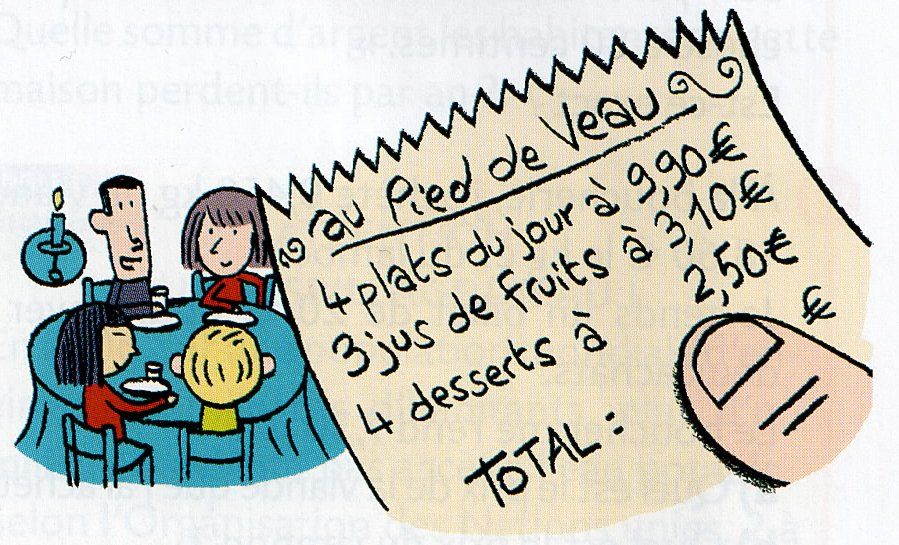
\includegraphics[width=7cm]{images/ex7.jpg}
\end{minipage}
\end{tabular}


\bigskip


\ul{Exercice 8}: (\textit{2 points})

\enskip

Pour fabriquer des rideaux, je choisis du tissu qui co�te 25,40 \euro le m�tre.
J'en ach�te 3,65m. Combien dois-je payer?
\end{document}
